% This is the chapter on sequencing and coverage analysis

\chapter{Sequencing}
\section{Experimental Design and Laboratory Workflow}
The primary objective of this research was to identify transcript boundaries and novel transcripts. A strand-specific RNA sequencing approach is superior to array based approaches and standard RNA-seq for detecting strand specific signal at high resolution. Additionally, this technique offers true strand specific signal, typically with 1-5\% background antisense signal. Therefore, this technique was selected for optimal resolution and sensitivity.

After selecting the appropriate technique, a range of experimental conditions was selected to best sample multiple times throughout the \textit{C. acetobutylicum} growth curve (\ref{fig:1}) and in response to two fermentation products, butyrate and butanol. This organism responds to resource limitation, acid/solvent stress, and intercellular signaling (sources???) by activating stress and sporulation systems. These networks are incomplete in \textit{C. acetobutylicum} (source??) and understanding of these systems benefit from the discovery of transcript boundaries. With the technique and conditions established, additional components of the laboratory workflow(\ref{fig:2}) were optimized, starting with RNA quality and purity.

\begin{figure}
\small
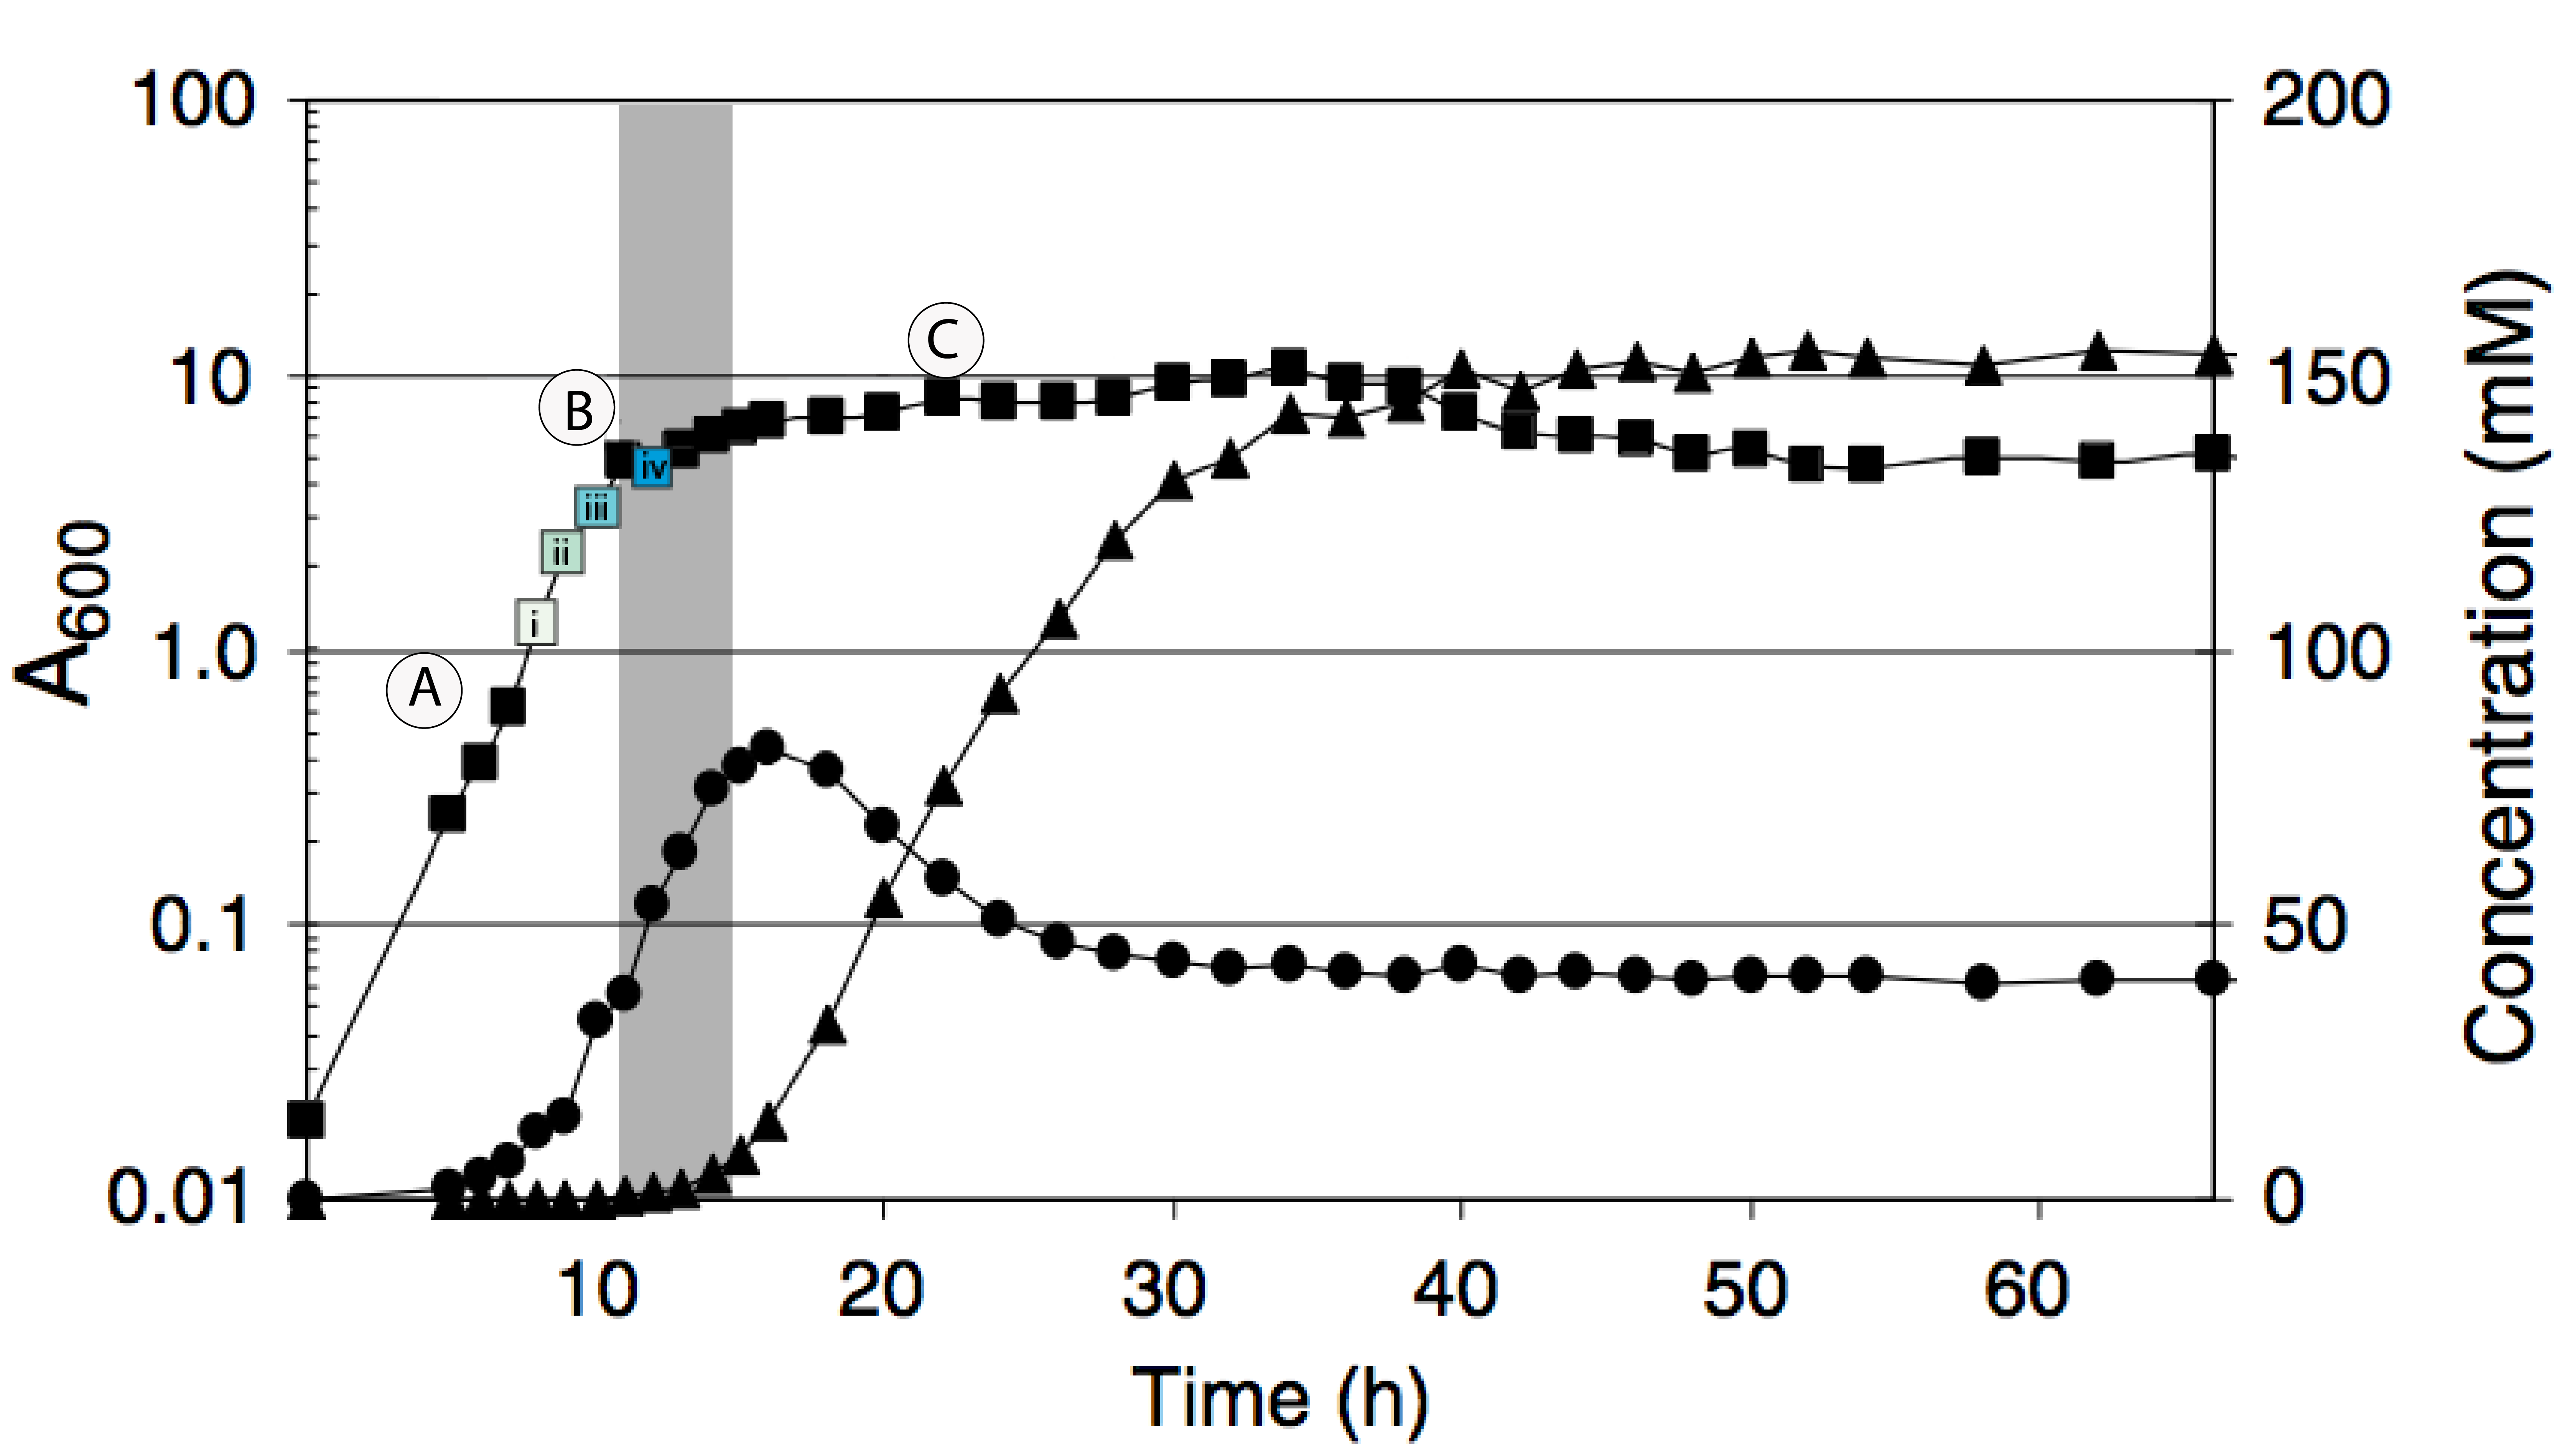
\includegraphics[width=\textwidth,height=3in]{images/Sequencing/Supplemental/Growth_curve.png}
\caption{\textit{C. acetobutylicum} Growth Curve}
\label{fig:1}
Populations of \textit{C. acetobutylicum} grow through the exponential phase ( A) A_{600} of 1.0), producing carboxylic acids, including butyric acid, during the transition phase (B). Then, the acids are reassimilated and reduced into solvents (C). These stressors were assayed in this experiment, in addition to time points 15(1.), 75(2.), 150(3.), and 270 minutes (4.) after synchronization at A_{600} of 1.0.
\end{figure}

RNA purity and integrity effect data quality. DNA contamination could effect the level of background signal. Small molecule, protein, or divalent cation contamination could degrade RNA or alter the effectiveness of the enzymatic reactions used in the preparation. RNA degradation effects the ultimate complexity of the library. To ensure RNA purity, after each step of RNA manipulation, the RNA was washed twice with 70\% alcohol, precipitated, and analyzed via spectrophotometry and the Agilent BioAnalyzer platform (\ref{methods:RNA_prep}). Ratios of absorbance ($\sfrac{\SI{260}{\nano\meter}}{\SI{280}{\nano\meter}}$, $\sfrac{\SI{260}{\nano\meter}}{\SI{230}{\nano\meter}}$) are frequently used to describe the purity of nucleic acid samples, due to purine/pyrimidine absorbance maxima at \SI{260}{\nano\meter}. Ratios of 2.0 indicate pure RNA, optimal for RNA-seq.

\begin{figure}
\hbox to \textwidth{\hfill
\rotatebox{90}{%
\begin{minipage}{\textheight}
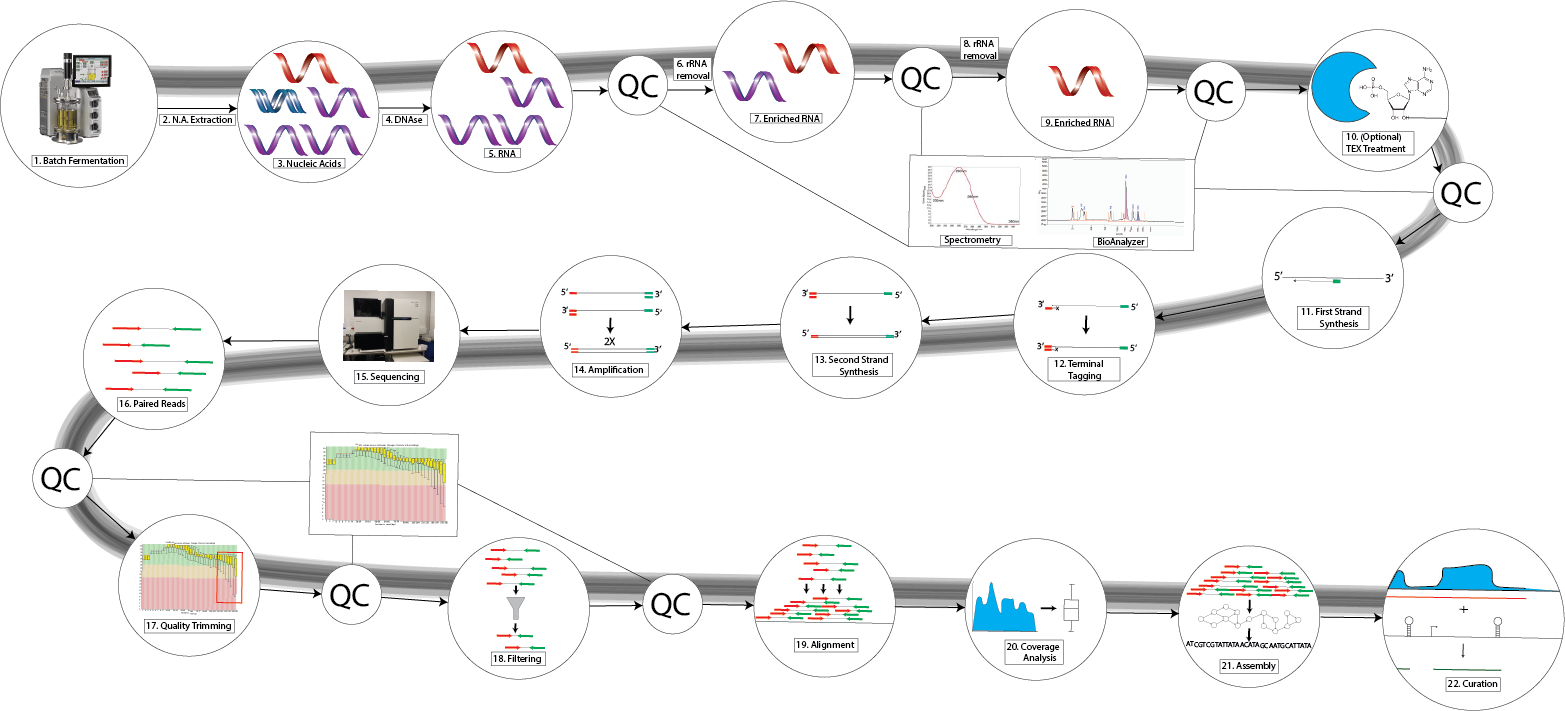
\includegraphics[width=\textheight,height=5in]{images/Sequencing/Supplemental/Workflow.png}
\caption{Laboratory Workflow}\label{fig:2}
The laboratory workflow consisted of mRNA enrichment steps and quality control analyses to ensure RNA quality. Ligation-free library preparation resulted in paired-end Illumina reads for preprocessing, alignment, analysis, and assembly.
\end{minipage}}\hfill}
\end{figure}

RNA integrity is commonly analyzed by interpreting ribosomal RNA bands. Specifically, a small peak width of the rRNA electrophoretic bands with little background signal indicates that the RNA high quality (e.g. RNA Integrity Number). A representative electropherogram is shown in \ref{fig:3}. The results clearly indicated high quality RNA with sharp, thin peaks for the 16S and 23S rRNA bands. With intact RNA, clear pellets, and clean spectrophotometric ratios, the RNA were then used for library preparation and sequencing. 

\begin{figure}
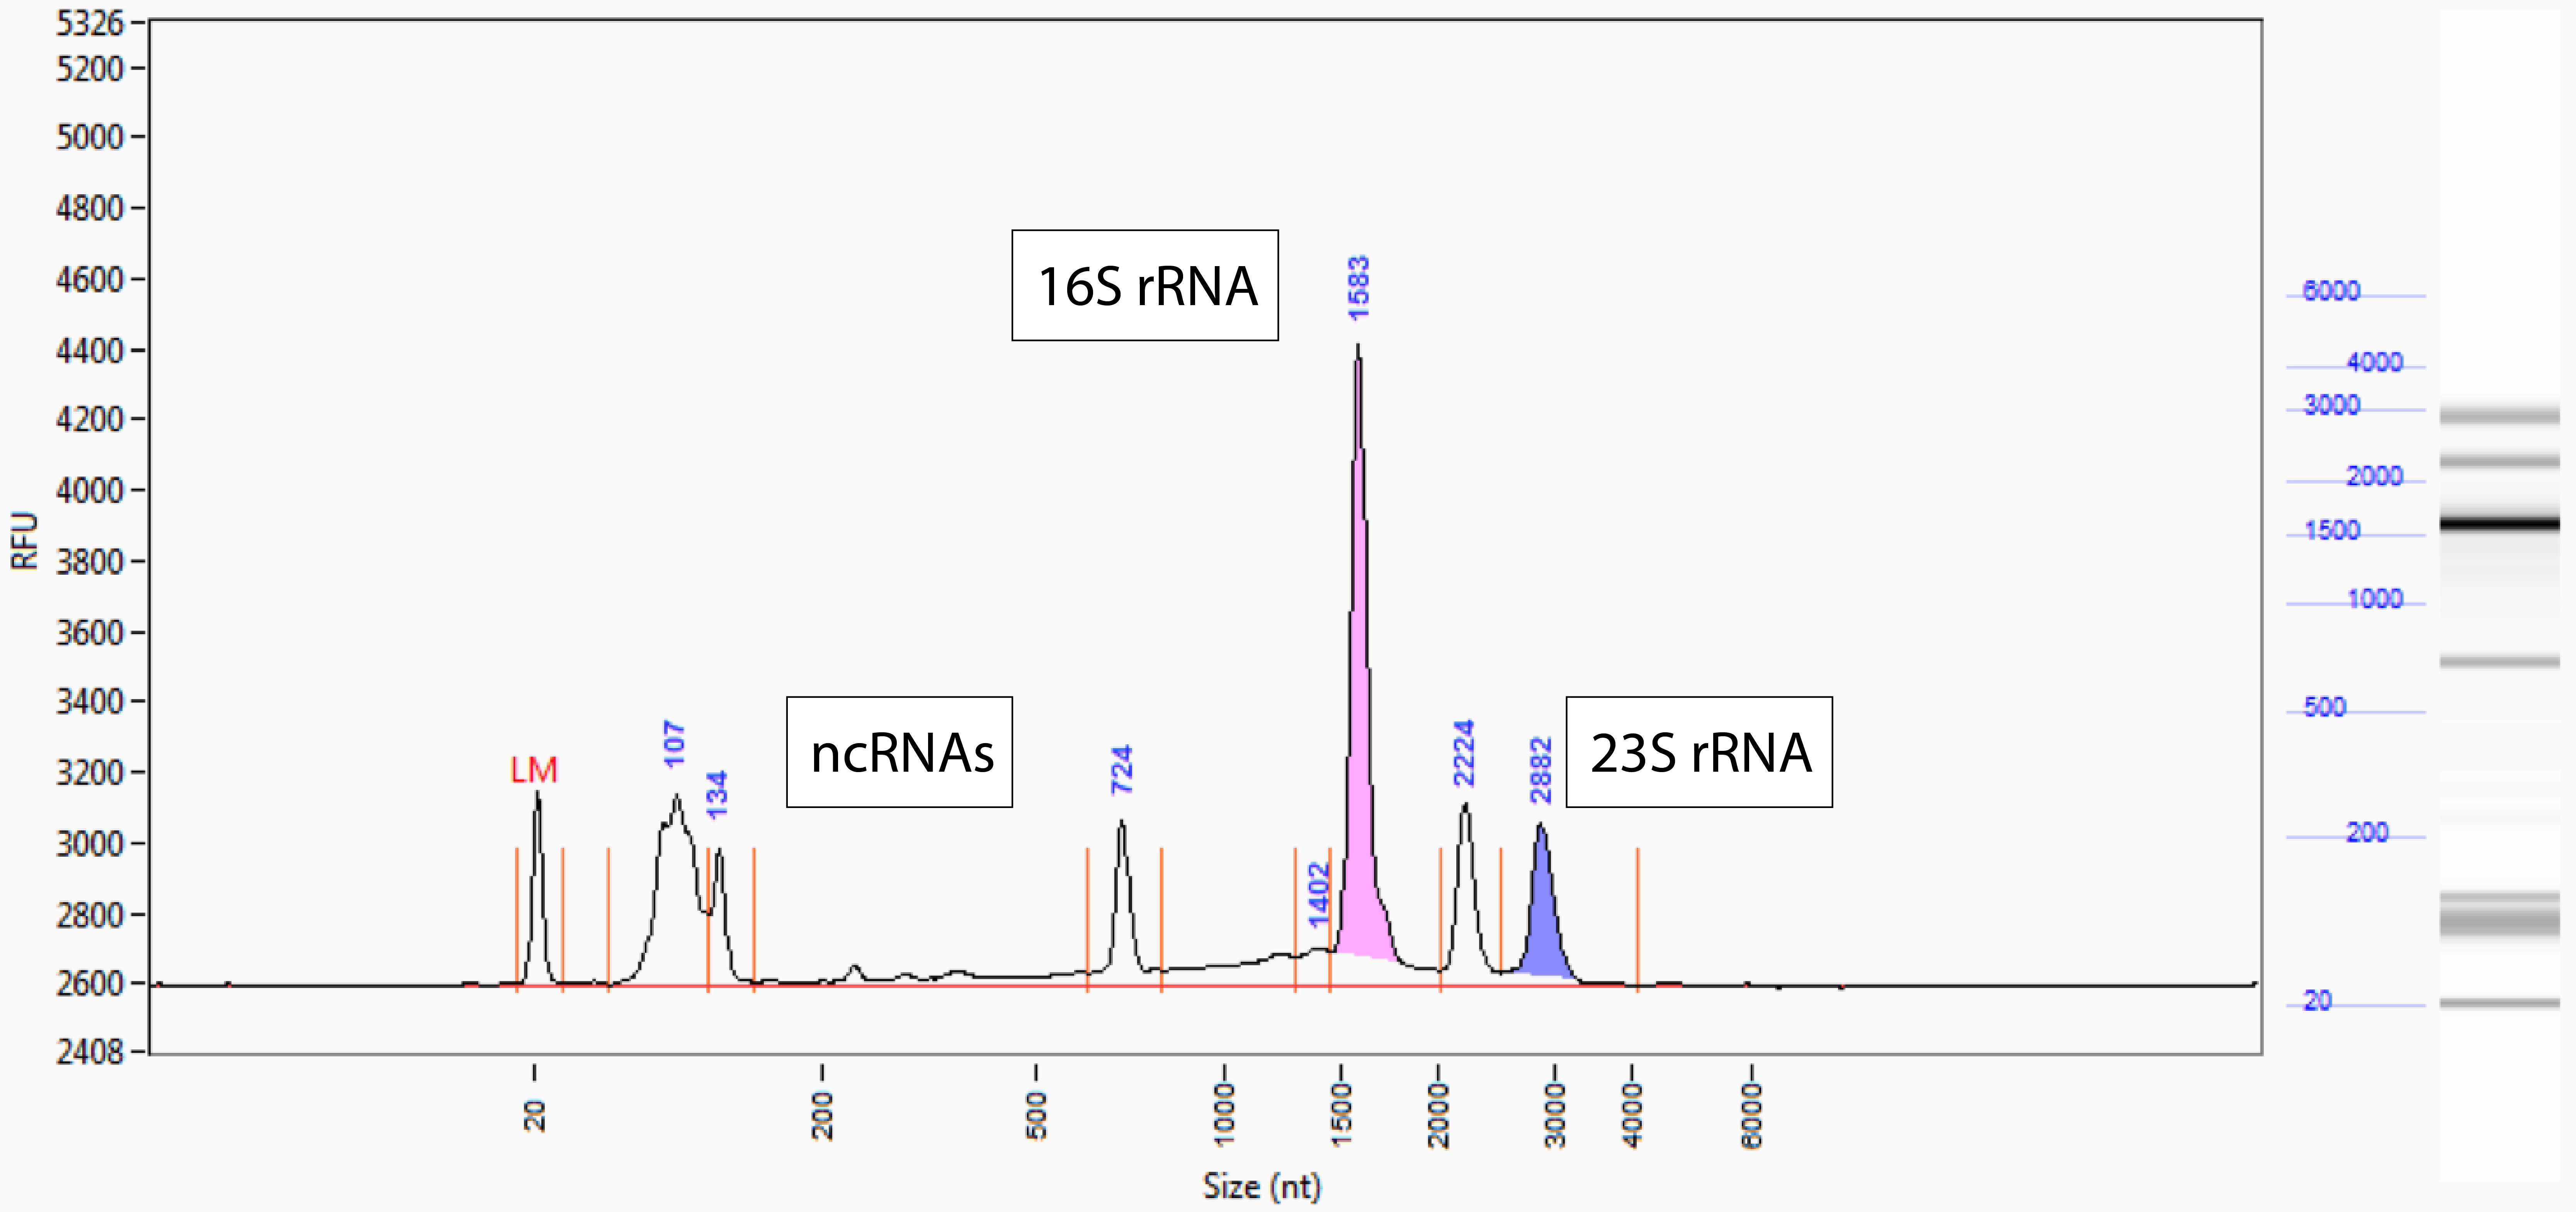
\includegraphics[width=\textwidth,height=3in]{images/Sequencing/Supplemental/RNA-integrity.png}
\caption{RNA Quality}\label{fig:3}
\end{figure}

\section{Data Processing, Alignment, and Coverage Analysis}
The libraries were sequenced paired-end over 6 lanes of an Illumina HiSeq 2500, producing 1.5 billion 75bp reads, averaging 25 million clusters/pairs per library. The reads were then processed through a customized bioinformatic workflow (\ref{methods:data_proc_aln}), first trimming low-quality bases, then filtering ribosomal RNA reads, and finally aligning to the genome (\ref{fig:2}). On average, 97\% of the useful, non-ribosomal reads were aligned to the \textit{C. acetobutylicum} genome. Of these, 7.75M(83\%) were properly paired, that is, both mates of each pair were in the correct orientation. In total, 458,814,860 perfectly paired reads were produced and then used for subsequent analysis. 

\newgeometry{left=2cm,right=2cm,top=1cm,bottom=1.5cm}
% Reads per library table
\begin{table}
%\hbox to \textwidth{\hfill
\rotatebox{90}{%
\begin{minipage}{\textheight}
\caption[Read Summary]{Read Summary}
\begin{tabular}{|l| *{12}{c|} }\hline%
ID & Stress & Time & Rep. & Barcode & Lane & Total & rRNA & non-rRNA & Mapped & Chrom. & pSol1 & Proper-pairs\\\hline\hline
\csvreader[late after line=\\\hline]%
{tables/Reads_Summary.csv}
{id=\id, stress=\stress,time=\time,replicate=\replicate,barcode=\barcode,lanes=\lanes,total=\total,rRNA=\rRNA,nonrRNA=\nonrRNA,mapped=\mapped,chromosomal=\chromosomal,pSol1=\pSol1,properlypaired=\properlypaired}{\id & \stress & \time & \replicate & \barcode & \lanes & \total & \rRNA & \nonrRNA & \mapped & \chromosomal & \pSol1 & \properlypaired}
%{id=\id, stress=\stress, time=\time, replicate=\replicate, barcode=\barcode, lanes=\lanes, total=\total, rrna=\rRNA, nonrrna=\nonrRNA, mapped=\mapped, chromosomal=\chromosomal, psol1=\pSol1, properlypaired=\properlypaired}%
%{\id & \stress & \time & \replicate & \barcode & \lanes & \total & \rRNA & \nonrRNA & \mapped & \chromosomal & \pSol1 & \properlypaired}%
\end{tabular}
\end{minipage}}
%\hfill}
\end{table}
\restoregeometry
%\csvautotabular{tables/Reads_summary.csv}



%\begin{figure}
%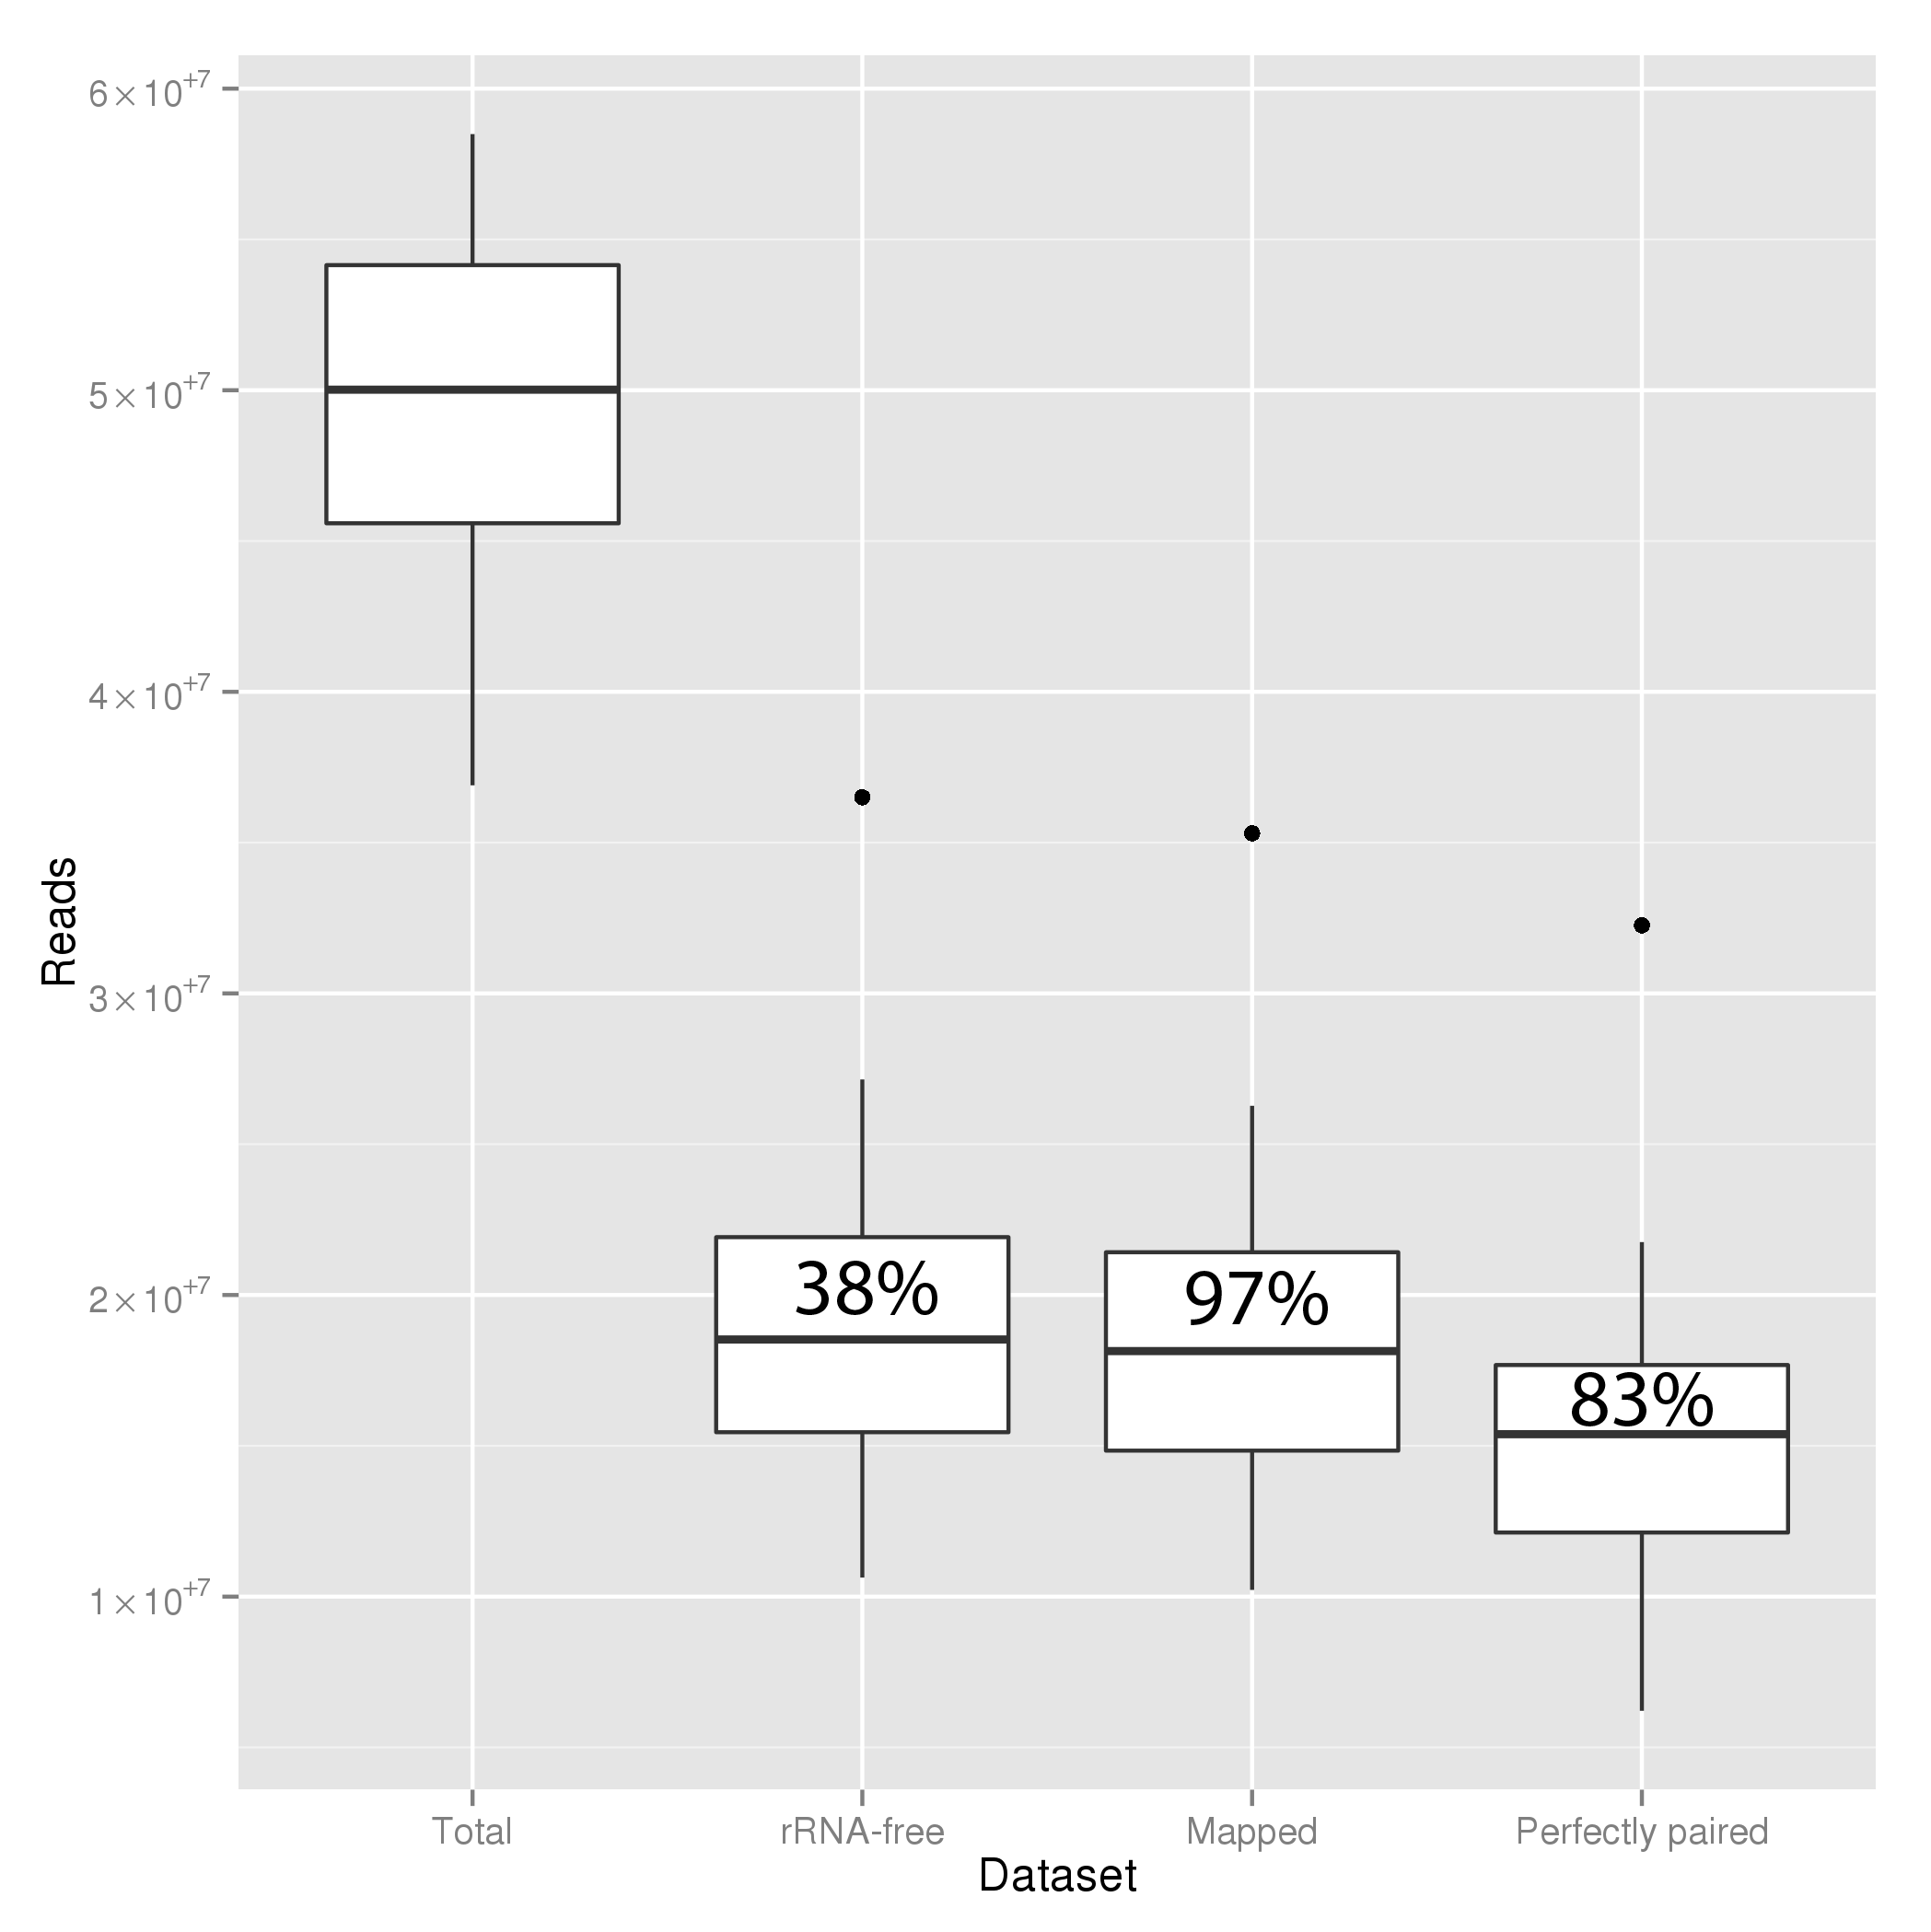
\includegraphics[width=\textwidth,height=3in]{images/Sequencing/Alignment_brief.png}
%\caption{Sequence Read Processing and Alignment}\label{fig:4}
%An average of 50 million reads (25M clusters/pairs) was produced for each of the 30 libraries. Ribosomal RNA reads were then filtered and the remaining reads were then aligned to the genome. Of these, 83\% were properly paired reads, ideal for transcriptome assembly.
%\end{figure}

After read alignment, it was desirable to determine the per base sequencing coverage across the genome.  The Encyclopedia of DNA Elements (ENCODE) project has released best practices guidelines for RNA-seq projects (Source??). Empirically, it seems that a coverage of 100-200M 100bp paired-end reads is sufficient to detect low abundance transcripts in the 60-140 megabases(Mb) hg19 human transcriptome. This sums to 20-40Gb of sequencing, 120-660x through a back of the envelope calculation, with a very conservative estimate of the size of the human transcriptome. In the case of \textit{C. acetobutylicum}, the upper boundary on the transcriptome is 8.2Mb, with a realistic estimate between 4-6Mb. With just the properly paired reads, 68.7Gb were sequenced for a much smaller transcriptome, approximately 11-17k times the length of the transcriptome. This estimate suggests that cumulatively, this study achieves comparable or superior depth than recommended by these guidelines. 

However, this estimate poorly represents the actual distribution of coverage per base throughout the transcriptome. A median of > 10x coverage per base and per strand was observed for each of the 30 libraries (ref{fig:5a}). Cumulatively, the median per base coverage is 156x throughout the genome(ref{fig:5b}). It is likely that in truly transcribed regions, the coverage is greater. Rather, some of the coverage described by this distribution is likely due to background signals from the RNA-seq technique. Background signal is indeed a pressing concern for RNA-seq (ENCODE source), potentiall from residual DNA escaping the RNA purification, DNAse digestion, and spectrophotometric analyses of the laboratory workflow. 


%\begin{figure}
%{\includegraphics[width=\textwidth,height=3in]{images/Sequencing/Example_coveragepng}
%\subcaption{Representative Genome Coverage Distribution}\label{fig:5a}}
%{\includegraphics[width=\textwidth,height=3in]{images/Sequencing/Cumulative coverage.png}
%\subcaption{Cumulative Genome Coverage Distribution}\label{fig:5b}}
%\caption{Coverage Boxplots}
%\subref{fig:5a}) Initial co
%\end{figure}


